\chapter{مروری بر کارهای پیشین}

\section{مقدمه}
در این فصل، به مرور کارهای گذشته می پردازیم.
مدل سیستم مقالات مختلف را معرفی کرده و مورد بررسی قرار می دهیم و نتایج عددی آن را نیز با یکدیگر مقایسه می نماییم.
\section{ شبکه های دسترسی رادیویی ابری}
شبکه های دسترسی رادیویی ابر (C-RAN) به عنوان یک چارچوب امیدوار کننده برای سیستم های ارتباط بی سیم نسل پنجم ظاهر شده اند.
از آنجا که آنها می توانند پیچیدگی رمزگشایی، مصرف انرژی و دخالت های ناشی از افزایش تراکم تلفن همراه را کاهش دهند\cite{cranInt}.
در ادامه در مورد برش شبکه در بخش رادیویی شبکه های دسترسی رادیویی ابری صحبت می کنیم.
\subsection{برش شبکه در شبکه های دسترسی رادیویی ابری}
در مقاله ی \cite{lee2018dynamic}
برش شبکه به صورت دینامیکی در بخش رادیویی مورد بررسی قرار گرفته شده است.
چارچوب طرح برش شبکه شامل یک سطح بالاتر، که مدیریت کنترل پذیرش، تشکل و تخصیص منابع باند پایه و یک سطح پایین تر، که تخصیص منابع رادیو در میان کاربران می باشد.
در این مدل فرض می کنیم که هر سرویس دارای شبکه اصلی خود (یا قطعه اصلی شبکه) است که به H-CRAN متصل می شود.
سلول بزرگ RRH (M-RRH) و سلولهای کوچک RRHs (S-RRHs) به ترتیب از طریق پیوندهای پشتی و fronthaul به یک استخر ابر
BBU  متصل می شوند.
همچنین ، تقسیم C/U در مدل سیستم فرض می شود، که به موجب آن صفحات کنترل و داده از هم جدا می شوند به گونه ای که صفحات کنترل توسط M-RRH در شبکه مدیریت می شود.
\begin{figure}[H]
  \centering
    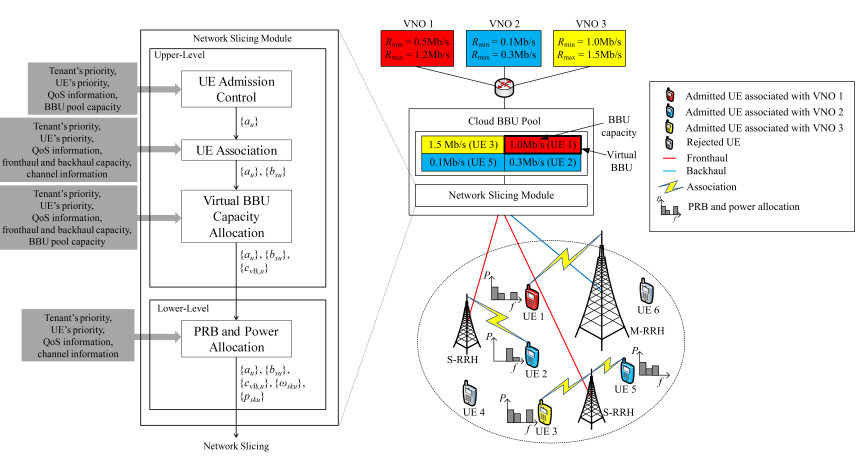
\includegraphics[scale = 0.7]{./fig/dynamicNS}
  \caption{روند برش شبکه\ \cite{lee2018dynamic}}
  \label{fig:dns}
\end{figure}
%برای حل این مسئله، می بایست مسئله را به بخش های کوچکتر تقسیم کرده و حل نماییم.
همانطور که در شکل \eqref{fig:dns} 
مشخص شده است ابتدا پذیرش کاربر مورد توجه قرار می گیرد و سپس کاربر به RRH متصل می شود و پس از آن ظرفیت BBU به آن تخصیص می دهد که تا این بخش از کار در سطح بالا قرار داریم.
در سطح بالا، یک مسئله کنترل پذیرش با برنامه نویسی پویا می باشد که در آن می توان پیچیدگی را می توان تنظیم کرد.
همچنین مسئله ی ارتباط کاربر با استفاده از یک الگوریتم حریص با پیچیدگی کم بهینه و حل می شود.
 مسئلهی تخصیص ظرفیت BBU نیز فرموله شده و با برنامه ریزی خطی حل می شود.
 حال وارد الگوریتم سطح پایین تر می شویم که تخصیص توان و منبع فیزیکی می باشد.
برای مساله ی سطح پایین تر، مشکل تخصیص منابع به عنوان یک مشکل برنامه نویسی mixedinteger غیر محدب است که با استفاده از روش دوگانه لاگرانژ حل می شود.


در مقاله ی 
\cite{larsen2018fronthaul,costanzo2018network}
برش شبکه در شبکه های دسترسی رادیویی ابری متوجه قرار گرفته است. 
در بخش fronthaul شبکه مشکلاتی از قبیل پیچیدگی شبکه و محدودیت نرخ وجود دارد که در برش شبکه، منجر به بهبود آن می شود.
علاوه بر این ، C-RAN می تواند مجازی سازی مجموعه ای از توابع RAN را امکان پذیر کرده و راه را برای اصطلاحاً RAN مجازی باز کند. با این کار می توان چندین شبکه مجازی یا برش ایجاد کند.


در مقاله ی 
\cite{fran}
برش شبکه در بخش رادیویی برای ساختار مه \LTRfootnote{Fog Radio Access Network}
 یا F-RAN
  در نظر گرفته شده است که در آن دو نمونه برش شبکه برای هات اسپات و سناریوهای وسیله نقلیه با زیرساخت مربوط تنظیم می شود. به طور خاص ، چارچوب برای برش RAN به عنوان یک مشکل بهینه سازی مشترک برای مقابله با ذخیره کردن و انتخاب حالت است.
  با توجه به خواسته های کاربران مختلف و منابع محدود، پیچیدگی مسئله بهینه سازی اصلی بسیار زیاد است و همین امر باعث می شود که رویکردهای بهینه سازی سنتی به طور مستقیم سخت باشد.
 برای مقابله با این معضل ، یک الگوریتم یادگیری تقویت عمیق ارائه شده است ، که ایده اصلی آن این است که سرور ابر تصمیمات صحیحی را در زمینه ذخیره محتوا و انتخاب حالت برای به حداکثر رساندن عملکرد پاداش در وضعیت کانال پویا و وضعیت حافظه نهان ارائه می دهد.
 